\documentclass[aspectratio=169]{beamer}
\usepackage{tikz}
\usetikzlibrary{shapes.geometric}
\usepackage{amsmath,amssymb}

\setbeamertemplate{footline}[frame number]
\setbeamertemplate{navigation symbols}{}

\setbeamercolor{palette primary}{fg=black,bg=white}
\setbeamercolor{palette secondary}{fg=black,bg=white}
\setbeamercolor{structure}{fg=black,bg=white}

% title frame
\defbeamertemplate*{title page}{mytheme}[1][]
{
  \begin{tikzpicture}[remember picture,overlay]
  \filldraw[white]
    (current page.north west) --
    (current page.north east) --
    ([xshift=0cm,yshift=-2cm]current page.north east)  --
    ([xshift=0cm,yshift=-2cm]current page.north west) -- cycle
    ;
  
  \node[opacity=0.2] at ([xshift=-1.5cm,yshift=-1cm]current page.north east) {\includegraphics[width=15cm]{monkon}};
  
  \node[text=black,anchor=south west,font=\sffamily\LARGE,text width=.8\paperwidth] at ([xshift=-100pt,yshift=-1cm]current page.center)(title){\raggedright\inserttitle};
    
  \node[text=black,anchor=south west,font=\sffamily\small,text width=.6\paperwidth] at ([xshift=-100pt,yshift=-1.5cm]current page.center)(institute){\raggedright\insertinstitute};
   
  \node[text=black,font=\large\sffamily,anchor=south west] at ([xshift=30pt,yshift=0.5cm]current page.south west)(date){\insertdate};
  
  \node[text=black,font=\large\sffamily,anchor=south west] at ([yshift=5pt]date.north west)(author){\insertauthor};
  \end{tikzpicture}
}

% definition of the symbols used in itemize
\newcommand\mysymbol{%
  \begin{tikzpicture}[xscale=0.85]
\draw[black, thick]  circle (1.5 pt);             
  \end{tikzpicture}%
  }

% definition of the itemize templates
\defbeamertemplate*{itemize item}{mysymbol}{\small\raise0.5pt\hbox{\mysymbol}}
\defbeamertemplate*{itemize subitem}{mysymbol}{\footnotesize\raise0.5pt\hbox{\mysymbol}}
\defbeamertemplate*{itemize subsubitem}{mysymbol}{\footnotesize\raise0.5pt\hbox{\mysymbol}}

\title[Transaction efficiency then and now]{Transaction efficiency then and now}
\author{Sarang Noether, Ph.D.}
\date{23 June 2019}

\institute{Monero Konferenco}

\begin{document}

\begin{frame}[plain]
\maketitle
\end{frame}


\begin{frame}
\frametitle{Disclaimer}
\begin{columns}
\begin{column}{0.2\textwidth}
\includegraphics[width=0.9\textwidth]{monero.png}
\end{column}
\begin{column}{0.8\textwidth}
The views expressed in this presentation are solely those of the author, and do not necessarily reflect those of any other person, organization, or community. \\~\\

The author receives funding support from the Monero community.
\end{column}
\end{columns}
\end{frame}


\begin{frame}
\frametitle{What is transaction efficiency?}
\begin{columns}

\begin{column}{0.3\textwidth}
\centering
\includegraphics[width=0.4\textwidth]{icon-space.png} \\~\\
\textbf{Space} \\
Bandwidth/storage
\end{column}

\begin{column}{0.3\textwidth}
\centering
\includegraphics[width=0.4\textwidth]{icon-hourglass.png} \\~\\
\textbf{Generation time} \\
Low-capacity devices
\end{column}

\begin{column}{0.3\textwidth}
\centering
\includegraphics[width=0.4\textwidth]{icon-stopwatch.png} \\~\\
\textbf{Verification time} \\
Chain sync
\end{column}

\end{columns}
\end{frame}


\begin{frame}{Levels of optimization}
\begin{columns}
\begin{column}{0.5\textwidth}
We can optimize at difference levels:
\begin{itemize}
\item low-level cryptographic operations
\item higher-level constructions
\item protocol parameters \\~\\
\end{itemize}

We will focus on \textit{constructions} today, but all of these have effects.
\end{column}
\begin{column}{0.5\textwidth}
\centering
\includegraphics[width=0.9\textwidth]{chain-growth.pdf} \\
Chain growth over time
\end{column}
\end{columns}
\end{frame}


\begin{frame}
\begin{figure}
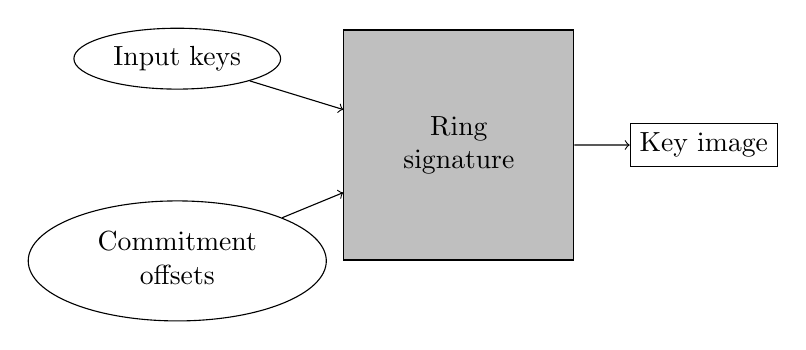
\begin{tikzpicture}[square/.style={regular polygon,regular polygon sides=4}]
\node [square,draw,fill=lightgray] (sig) {\begin{tabular}{c}Ring \\ signature\end{tabular}};
\node [ellipse,draw,left=60pt,at=(sig.west),above=20pt] (inputs) {Input keys};
\node [ellipse,draw,left=60pt,at=(sig.west),below=20pt] (offsets) {\begin{tabular}{c}Commitment \\ offsets\end{tabular}};
\node [rectangle,draw,right=20pt,at=(sig.east)] (image) {Key image};

\draw [->] (inputs) -- (sig);
\draw [->] (offsets) -- (sig);
\draw [->] (sig) -- (image);
\end{tikzpicture}
\end{figure}
\centering
The ring signature proves key ownership, helps demonstrate transaction balance, and asserts correct key image construction.
\end{frame}


\begin{frame}
\begin{figure}
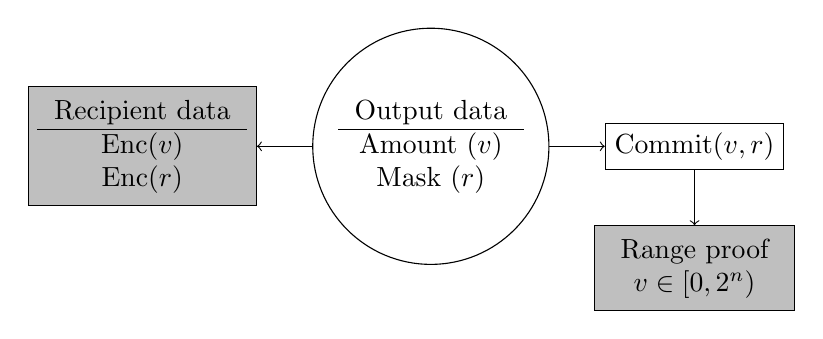
\begin{tikzpicture}[square/.style={regular polygon,regular polygon sides=4}]
\node [circle,draw] (data) {\begin{tabular}{c}Output data \\ \hline Amount ($v$)\\ Mask ($r$)\end{tabular}};
\node [rectangle,draw,left=20pt,at=(data.west),fill=lightgray] (enc) {\begin{tabular}{c}Recipient data \\ \hline $\operatorname{Enc}(v)$ \\ $\operatorname{Enc}(r)$\end{tabular}};
\node [rectangle,draw,right=20pt,at=(data.east)] (commit) {$\operatorname{Commit}(v,r)$};
\node [rectangle,draw,below=20pt,at=(commit.south),fill=lightgray] (range) {\begin{tabular}{c}Range proof \\ $v \in [0,2^n)$\end{tabular}};

\draw [->] (data) -- (enc);
\draw [->] (data) -- (commit);
\draw [->] (commit) -- (range);
\end{tikzpicture}
\end{figure}
\centering
The output constructions communicate output data to the recipient, are used (with auxiliary commitments) to show balance, and prevent amount overflow.
\end{frame}


\begin{frame}{Construction: ring signature}
We use \textbf{MLSAG} signatures to prove ownership of spent outputs without revealing the specific output in question. This type of ring signature shows more, though.
\begin{itemize}
\item The signer controls one output among a given set
\item The key image (used to detect double-spend attempts) was generated correctly
\item The (hidden) transaction amounts balance \\~\\
\end{itemize}

These signatures scale \textit{linearly} with the ring size in space, signing time, and verify time.
\end{frame}


\begin{frame}{CLSAG: the new hotness}
We propose \textbf{CLSAG} signatures to do the same thing, but more efficiently. \\~\\

CLSAG signatures use a linear combination of output signing keys and commitment keys to provide a drop-in replacement to MLSAG signatures. \\~\\

They still scale linearly, but take up less space and are faster to sign and verify. \\~\\

Security is more formally proven.
\end{frame}


\begin{frame}{Signature size (11-ring)}
\centering
\includegraphics[width=0.7\textwidth]{sig-size.pdf}
\end{frame}


\begin{frame}{Timing (11-ring)}
\begin{columns}
\begin{column}{0.5\textwidth}
\centering
\includegraphics[width=\textwidth]{sig-sign.pdf} \\~\\
\textbf{Signing}
\end{column}
\begin{column}{0.5\textwidth}
\centering
\includegraphics[width=\textwidth]{sig-verify.pdf} \\~\\
\textbf{Verification}
\end{column}
\end{columns}
\end{frame}


\begin{frame}{Construction: commitments}
All amounts are represented as Pedersen commitments with globally fixed base:
$$\operatorname{Commit}(v,r) \equiv \underbrace{vH}_{\text{value}} + \underbrace{rG}_{\text{mask}}$$

The recipient needs to know both $v$ and $r$ to reconstruct the commitment and later use it in a ring signature to spend the output. \\~\\

Previously, both values were encrypted using the transaction shared secret $\operatorname{H}(aR,i)$:
\begin{eqnarray*}
\operatorname{Enc}(v) &\equiv& v + \operatorname{H}(\operatorname{H}(\operatorname{H}(aR,i))) \\
\operatorname{Enc}(r) &\equiv& r + \operatorname{H}(\operatorname{H}(aR,i))
\end{eqnarray*}
\end{frame}


\begin{frame}{New hotness: being clever}
\textbf{This is wasteful}. If generated randomly, both $r$ and $\operatorname{Enc}(r)$ are uniformly distributed and known only to the sender and recipient. So why include $\operatorname{Enc}(r)$ in the transaction at all? \\~\\

\textbf{Solution}: Do not include $\operatorname{Enc}(r)$. The sender and recipient both compute $$r \equiv \operatorname{H}(``\text{commitment\_mask}",\operatorname{H}(aR,i))$$ instead, and save $32$ bytes per output. \\~\\
\end{frame}


\begin{frame}{New hotness: being clever}
\textbf{This is still wasteful}. The amount cannot be larger than $8$ bytes, but is represented as a $32$-byte scalar. \\~\\

\textbf{Solution}: Restrict the amount representation to $8$ bytes and encrypt with a length-restricted XOR operation to save $24$ bytes per output:

$$\operatorname{Enc}(v) \equiv \Big( v \oplus \operatorname{H}(``\text{amount}",\operatorname{H}(aR,i)) \Big)_{0-7}$$

The full 32-byte scalar can be recovered in the same way.
\end{frame}


\begin{frame}{Commitment data size}
\centering
\includegraphics[width=0.7\textwidth]{commit.pdf}
\end{frame}


\begin{frame}{Construction: range proofs}
Since amounts are represented as commitments and balance is proven using commitment sums and differences, amounts must be restricted (relative to scalar field size) to avoid overflow. \\~\\

We must show that for $\operatorname{Commit}(v,r)$, the value $v$ is in the range $[0,2^{64})$. \\~\\

\textbf{Strategy}: Show that $v$ can be decomposed to $64$ bits, each of which is $0$ or $1$, without revealing the value of the bits. \\~\\

\textbf{Example}: $13_{10} = 1101_2 = (1 \times 2^3) + (1 \times 2^2) + (0 \times 2^1) + (1 \times 2^0)$
\end{frame}


\begin{frame}{Old way: bitwise ring signatures}
The previous method, bitwise Borromean range proofs, used ring signatures.
\begin{itemize}
\item Construct $64$ commitments, each to a bit of $v$, with masks that sum appropriately.
\item Build a ring signature over each bit commitment to show the value is either $0$ or $1$. \\~\\
\end{itemize}

To verify:
\begin{itemize}
\item Take a weighted sum of the bit commitments (using powers of $2$) and show it recovers the full amount commitment.
\item Verify the ring signature to assert that each commitment is to $0$ or $1$. \\~\\
\end{itemize}

This scales in space and time linearly with the number of bits!
\end{frame}


\begin{frame}{Bulletproofs: the new hotness}
Bulletproofs take a different approach.
\begin{itemize}
\item Reduce the range assertion to a set of vector inner product equations.
\item Prove knowledge of vector components in zero knowledge.
\item Compress this proof using a clever folding technique. \\~\\
\end{itemize}

This achieves precisely the same goal as bitwise Borromean proofs, but scales logarithmically with the number of bits. Plus:
\begin{itemize}
\item A prover can include multiple values in the same proof, to extend the logarithmic space scaling.
\item Generation and verification are still linear in the bit length, but we can use tricks.
\item Verification of a set of proofs adds only marginal time cost! (This is \textit{batching}.)
\end{itemize}
\end{frame}


\begin{frame}{2-output verification}
\centering
\includegraphics[width=0.7\textwidth]{bp-2.pdf}
\end{frame}


\begin{frame}{16-output verification}
\centering
\includegraphics[width=0.7\textwidth]{bp-16.pdf}
\end{frame}


\begin{frame}{2-output 128-batch verification}
\centering
\includegraphics[width=0.7\textwidth]{bp-2-batch-128.pdf}
\end{frame}

\begin{frame}{Proof size}
\centering
\includegraphics[width=0.7\textwidth]{bp-size.pdf}
\end{frame}


\begin{frame}{Typical transaction}
\begin{columns}
\begin{column}{0.5\textwidth}
\centering
\includegraphics[width=\textwidth]{txn-size-2-2.pdf} \\~\\
\textbf{Transaction size}
\end{column}
\begin{column}{0.5\textwidth}
\centering
\includegraphics[width=\textwidth]{txn-time-2-2.pdf} \\~\\
\textbf{Verification time}
\end{column}
\end{columns}
\begin{center}
We save $85\%$ on space and up to $81\%$ on verification time!
\end{center}
\end{frame}


\begin{frame}
\begin{center}
\textbf{These are not complete scaling solutions!}
\end{center}

These are incremental (but useful) improvements to slow blockchain growth and speed up new node sync time. \\~\\

\begin{itemize}
\item Sublinear fixed-decoy transaction protocols
\begin{itemize}
\item Lelantus
\item Omniring
\end{itemize}
\item Efficient full-anonymity transaction protocols
\begin{itemize}
\item Bulletproofs (poor verification scaling for circuits)
\item Older-style SNARKs (toxic; excellent space/time scaling)
\item Newer-style SNARKs (nontoxic; better scaling, but not quite there)
\end{itemize}
\item Off-chain transaction layers (requires new plumbing)
\begin{itemize}
\item Atomic swaps
\item Payment channels/networks
\end{itemize}
\end{itemize}
\end{frame}


\begin{frame}{Thank you!}
\textbf{GitHub}: \texttt{https://github.com/SarangNoether}
\begin{itemize}
\item \texttt{research-lab}: older research
\item \texttt{skunkworks}: newer research (work in branches) \\~\\
\end{itemize}

\textbf{GitLab}: \texttt{https://repo.getmonero.org/SarangNoether}
\end{frame}

\end{document}